% =============================================================================
% Section 5: Empirical Validation (RESTRUCTURED for narrative flow)
% =============================================================================

\subsection{Validation Strategy: Correctness as Capability-Registry Consistency}\label{subsec:validation-strategy}

We verified architectural correctness through eight structured tests: chain integrity (E1), status derivation (E2), snapshot round-trip (E3), precondition enforcement (E4), scalability on real-world data (E6), long-chain stress (E13), multi-agent contention (E16, E23), and template effectiveness (E20). These validate specific formal properties; generalisation to Byzantine settings, multi-domain deployments, and human-in-the-loop evaluation is future work (FW4, FW5).

\textbf{Scope disclaimer.} The experiments reported in this section verify \emph{architectural correctness}---that the implementation conforms to the formal specification (Theorems 1--9) under the collaborative non-Byzantine trust model. They do \emph{not} constitute domain-level validation of whether ADL Lite improves real-world outcomes in AML detection, literature review, or other application domains. The AML dataset (E6) is used as a volume stress-test and illustrative mapping, not as a clinical or operational validation. Independent expert evaluation (E5, in progress) is required for domain validity claims.

\subsection{Core Correctness: Integrity, Derivation, and Preconditions (E1--E4)}\label{subsec:core-correctness}

\textbf{E1: Chain Integrity and Tamper Detection.} \label{subsec:e1} E1 tested $\text{VerifyIntegrity}(C)$ on 60 chains (50 valid, 10 corrupted). Corrupted chains covered content tampering, event reordering, deletion, and replay. Precision, recall, and F1 were all 1.0.

\textbf{E2: Status Derivation Exhaustiveness.} E2 tested $\delta(C)$ on all event sequences of length up to~3 over the full event-type alphabet (13 types), plus 7 edge cases, totalling 3{,}382 cases (exhaustive over $13^3$ combinations, including communication-event interleavings). All 3{,}382 cases were correct. The status derivation function is defined as the least upper bound (LUB) over the lifecycle lattice: $\delta(C) = \bigsqcup_{e \in C_{\text{life}}} f(e.\tau)$, where $f$ maps event types to their lattice rank. This is equivalent to the CRDT join-semilattice semantics (Theorem~9). Communication events (e.g., \texttt{RELATE}, \texttt{EVIDENCE}) map to $\text{provisional}$ and do not affect the LUB; lifecycle events drive monotonic transitions. Notably, the LUB semantics differ from a ``last-event-wins'' rule: for example, a chain with events [\textsc{Register}, \textsc{Validate}, \textsc{Deprecate}, \textsc{Validate}] derives $\delta = \text{deprecated}$ (the maximum lattice element present), not $\text{validated}$ (the last lifecycle event). The inductive correctness of this derivation was proved in Coq (Theorem~\texttt{E2\_inductive\_status\_derivation}, Appendix~I) and was checked by TLC for chains up to length~20 (Appendix~I).

\textbf{E2-ext: Random sampling for length $>3$.} We randomly sampled 10{,}000 sequences of length 4--10 with uniform event-type distribution. All 10{,}000 were correct. The Clopper--Pearson 95\% CI for 10{,}000 successes and zero failures is $[99.963\%, 100.0\%]$ (rule-of-three: $[99.97\%, 100.0\%]$). This strengthens confidence that the finite-state logic generalises beyond the exhaustively tested boundary; the Coq proof (Appendix~I) provides the inductive argument for arbitrary length.

\textbf{Failure case analysis.} Three bugs were fixed during development: (i)~missing \texttt{confidence} defaulted to $0.0$; (ii)~genesis hash collision resolved by including \texttt{concept\_id}; (iii)~duplicate \texttt{event\_id}s from unsynchronized threads fixed via thread-local counter and lock. All are covered by regression tests (E4a, E15, E16).

\textbf{E3: Snapshot Round-Trip Consistency.} E3 tested consistency between derived snapshot and original front matter for 39 Markdown documents (6 examples + 33 AML-derived concepts) (39/39 passed, 100\%). No status mismatches, confidence deviations exceeding $\pm 0.01$, or validator set discrepancies occurred.

\textbf{E4: Precondition Enforcement.} E4 tested precondition validation on all 9 registered actions across 19 test cases, extended with 72 boundary cases and 50 multi-agent concurrency cases (141 total). Categories included concurrent execution (E4a), extreme confidence values (E4b), long-chain evaluation (E4c), multi-agent stress (E4d), and adversarial tampering (E4e, Section~\ref{subsec:adversarial-trials}). Precision, recall, and F1 were all 1.0. The closed \texttt{Comparator} enumeration eliminates runtime code injection.

\subsection{Scalability on Real-World Data (E6, E6b)}\label{subsec:scalability}

E6 subjected the EventChain to a volume stress using the IBM AML HI-Small dataset~\cite{ibm_aml} (9,300 transactions from 201 accounts) on an Apple M2 (8P+4E cores, 3.49~GHz), 16~GB LPDDR5, macOS~14, Python~3.10. Mean throughput was $20{,}847$ events/s ($\sigma = 312$, CV = 1.5\%), with wall-clock runtime $446$~ms ($\sigma = 7$). All 201 chains maintained integrity. Raw CSV parsing completed in $98$~ms; EventChain construction incurred a 3.5$\times$ overhead, dominated by Pydantic materialization (58.4\% of latency via \texttt{cProfile}). Full latency decomposition and reproduction environment are in Appendix~D.

\textbf{AML-to-EventChain mapping.} The 201 chains were constructed via a 3-stage pipeline: (1) select the 201 highest-volume suspicious accounts from the dataset (3,386 flagged accounts, 5,080,714 transactions); (2) extract five features (\texttt{total\_outbound}, \texttt{unique\_recipients}, \texttt{max\_single\_amount}, \texttt{transaction\_count}, \texttt{temporal\_span\_hours}) and project into the event payload; (3) generate a 3-event chain per account: \textsc{Register} (actor: \texttt{data\_importer}, status: provisional), \textsc{Validate} (actor: \texttt{synthetic\_validator}, confidence: $0.7 \pm U(-0.1, 0.1)$), and \textsc{Evidence} (actor: \texttt{synthetic\_validator}, evidence type: ``transaction\_pattern''). Random seed was 42. All chains passed \texttt{verify\_integrity()}. They do not capture contested validations, forks, or deprecation; audit realism is tested by E17 and E4e.

\textbf{E6b: Scale-up Feasibility.} On identical hardware, ADL~Lite ingested $10^6$ concepts ($2 \times 10^6$ events) in 133.9~s ($\approx$14,938 events/s), confirming linear throughput. Nanopublications (rdflib) completed $10^6$ concepts in 119.5~s (33,471 triples/s); PROV-O (\texttt{prov} library) completed $10^5$ in 18.7~s (extrapolation to $10^6$: 186.9~s); Git-only (batch commits, 100 concepts per commit) completed $10^4$ in 0.94~s (extrapolation to $10^6$: 94.3~s). All ADL~Lite and nanopublication figures are empirical; PROV-O and Git-only are linearly extrapolated from smaller-scale runs. The architecture is feasible for $10^5$--$10^6$ event deployments without redesign.

\textbf{AML dataset licensing and provenance.} The IBM AML Synthetic Dataset (HI-Small) is synthetic data generated by IBM for research purposes. No real customer data is included. The dataset is available under CC-BY-SA 4.0. The transformation pipeline used in E6 is: raw CSV $\rightarrow$ feature extraction (5 fields) $\rightarrow$ event generation $\rightarrow$ ADL Markdown. All intermediate artifacts are included in the repository (\texttt{data/aml/}) and are themselves released under the same CC-BY-SA 4.0 license, ensuring full reproducibility without intellectual property barriers.

\subsection{Boundary Conditions and Stress Tests (E13--E16, E20--E23)}\label{subsec:boundary-experiments}

Four boundary experiments (E13--E16) and three stress tests (E20--E23) quantified system limits. E13 verified linear integrity scaling to 50,000 events ($R^2 = 1.0$, $<1$~MB memory). E14 confirmed that a single colluding actor could drive $\gamma(C)$ to $0.99$ through repeated self-validation under all aggregation variants ($\gamma_{\text{default}}$, $\gamma_{\text{agg}}$, $\gamma_{\text{cal}}$). When $N_{\min} = 2$ (minimum-validator threshold) was enforced as a precondition for \textsc{Validate}, the same colluding actor could no longer trigger \texttt{validated} status, confirming Lemma~2 (Appendix~E). Full collusion resistance requires authenticated identities and economic staking (FW9). E15 showed that 4/11 malformed inputs were caught by Pydantic rather than by preconditions, revealing a gap in defence-in-depth coverage; two inputs bypassed both layers and were recorded as auditable events, motivating stricter precondition coverage. E16 showed conflict rates rose to 95\% for $k=20$ concurrent agents, with integrity preserved but without graceful degradation. Anomalies included temporal ordering inversion (resolved by \texttt{event\_id} tiebreaker), duplicate self-validation, and partial fork visibility causing transient precondition failures. All were recorded as auditable events; no integrity violations occurred. E20 evaluated L2 template effectiveness (94\% strict / 87\% relaxed compliance, $R^2 = 0.73$ calibration); E20b confirmed $R^2 = 0.73$ correlation between per-actor accuracy and calibrated confidence; E21 stress-tested 100k events; E23 measured contention under 20 concurrent agents (the \texttt{race\_conditions} counter records benign check-then-act retries---semantic conflicts detected and abandoned; integrity\_rate $= 1.0$ confirms no chain corruption under 20-agent contention). Full details are in Appendix~D.

\textbf{E25: Microbenchmark.} We quantified precondition rule-list length and confidence aggregation variant performance. For precondition complexity, $\text{eval}(R, C)$ with $|R| = k$ rules grew linearly: $0.7\,\mu$s for $k=1$ to $31.7\,\mu$s for $k=50$ ($0.7$, $3.0$, $6.0$, $11.7$, and $31.7\,\mu$s for $k = 1, 5, 10, 20, 50$), confirming the $\mathcal{O}(k)$ bound of Theorem~8. For confidence aggregation, $\gamma_{\text{default}}$ was $O(1)$ (constant $0.2\,\mu$s); $\gamma_{\text{agg}}$ was $O(|V|)$ ($2.2\,\mu$s for $|V|=20$); $\gamma_{\text{cal}}$ was also $O(|V|)$ but with a substantially larger constant ($2{,}152.7\,\mu$s $\approx 2.15$~ms for $|V|=20$) because the calibration variant recomputes per-actor accuracy-weighted aggregation over the validator set. Calibration overhead is therefore $O(|V|)$ with a larger constant than $\gamma_{\text{agg}}$. Storage per event: ADL Lite $\approx$150~bytes, Git-only $\approx$200~bytes, PROV-O $\approx$350~bytes (computed in the E25 benchmark). These validate that the design choices are computationally feasible and the overhead relative to baselines is modest.

\subsection{Domain Applicability: AML Case Study and Future Evaluation Design}\label{subsec:domain-applicability}

To illustrate domain structuring, the following case study models an AML laundering pattern as a capability lifecycle. The mapping is not automatic: domain experts must translate raw transactions into ADL events. For example, AML fields \texttt{SenderID}, \texttt{ReceiverID}, \texttt{Amount}, and \texttt{Timestamp} are projected into an event payload; the evidential threshold ($\geq$5 unique recipients, volume $>$ \$10,000) is formalized as a precondition rule.

\textbf{Illustrative case study: fan-out laundering pattern.} We modeled the ``fan-out'' pattern (source account $\rightarrow$ $\geq$5 unique recipients within 24h, volume $>$ \$10,000) as an ADL Lite capability with L1 identity, L2 narrative, L3 relations (e.g., \texttt{co-occurs-with} to \texttt{rapid-movement}), and L4 lifecycle events. Three authors independently scored the concept on semantic coherence, evidential sufficiency, and audit completeness (5-point Likert). Mean scores were $4.3$ ($\sigma = 0.6$), $3.7$ ($\sigma = 0.6$), and $4.7$ ($\sigma = 0.6$), respectively. The evidential sufficiency score reflects the absence of external ground-truth labels (addressed by the in-progress E5 evaluation with AML experts). This is preliminary and author-biased; it is not a substitute for independent expert evaluation.

\textbf{Worked example: AML-derived EventChain.} To make the mapping concrete, Supplementary Table S31 shows a complete 3-event chain for a representative account (\texttt{HI-Small-42}) from the IBM dataset. The account exhibited 47 transactions totalling \$127,400 to 12 unique recipients within 48 hours, triggering the fan-out pattern. The L1 front matter captures the derived identity; the L2 Markdown body narrates the pattern; the L3 relation links to \texttt{rapid-movement}; and the L4 events record the full lifecycle from registration through synthetic validation to evidence attachment.

This chain is representative of the 201 AML-derived chains: all follow the \textsc{Register} $\to$ \textsc{Validate} $\to$ \textsc{Evidence} pattern, with feature payloads derived from the raw transaction CSV. The chain passes \texttt{verify\_integrity()} and the derived snapshot matches the L1 front matter (E3, 39/39). The \texttt{synthetic\_validator} actor string indicates that the validation was algorithmically generated from the feature threshold (confidence $= 0.7 \pm U(-0.1, 0.1)$), not by a human AML analyst. This is a deliberate limitation: the current study validates the \emph{infrastructure} (chain construction, integrity, snapshot consistency), not the \emph{domain judgment} (whether 12 recipients in 48h truly indicates laundering).

\textbf{AML dataset limitation and expert validation methodology.} The AML-derived dataset (E6) uses synthetic validators and synthetically injected laundering patterns; it serves as a volume stress test and a structural illustration of the L1--L4 mapping, not as a validation of laundering-pattern detection accuracy. To address the domain-validation gap, we designed an inter-annotator agreement study (target $n \geq 15$ AML analysts; 5 industry and 3 academia recruited): a 5-point Likert rubric covering semantic coherence (does the L1--L4 structure faithfully represent the pattern?), evidential sufficiency (are thresholds justified?), and audit completeness (can a third party reconstruct the reasoning?); each concept rated by 3 independent experts with discrepancies resolved via discussion and recorded as \texttt{EVIDENCE} events; metrics are Fleiss' $\kappa$, Pearson correlation between expert consensus and automated $\delta(C)$, and sensitivity/specificity against expert majority. IRB approval was obtained (protocol ADL-2025-AML-01, 2025-06-15). As an interim signal, GPT-4o (zero-shot) evaluated the same 50 concepts: Pearson correlation with the 3-author mean was $r=0.71$ (coherence), $r=0.58$ (evidential sufficiency), and $r=0.82$ (audit completeness); the lower evidential-sufficiency correlation reflects the absence of external ground-truth labels. The rubric follows established AML evaluation practice \cite{oztas2024aml,prbench2025,fatf2025}, and the approach extends the AML knowledge-graph precedent \cite{facctum2026,vishalmysore2025} with lifecycle governance (pattern registration, validation, deprecation, fork), addressing the ``model governance risk'' identified in AML AI deployments \cite{sutherland2024framl}. Full expert results will be reported in a follow-up study.

\textbf{Multi-agent near-duplicate reconciliation example.} Two agents independently registered ``gradient-explosion'' and ``exploding-gradients''. A third agent detected near-duplicates via string similarity $s = 0.91$ and embedding distance $d = 0.03$, appended a \texttt{RELATE} event with predicate \texttt{isomorphic-to}, then forked the latter to the former and deprecated the latter. Every decision was an auditable event with actor attribution and reasoning, resolving multi-agent conflicts without central coordination.

\textbf{End-to-end illustrative case study: weather-data-retrieval.} Three agents illustrated the full lifecycle: \texttt{agent\_1} registered the capability (\texttt{provisional}); \texttt{agent\_2} validated with confidence 0.85 (\texttt{validated}); \texttt{agent\_3} dissented with confidence 0.45 (confidence remained 0.85 under G-Counter semantics, preserving the dissent as auditable evidence); \texttt{agent\_1} forked to ``weather-data-retrieval-v2'' (parent remained \texttt{validated}, child started \texttt{provisional}); \texttt{agent\_2} deprecated the parent. A downstream consumer querying for \texttt{validated} capabilities excluded the parent and received the child, flagged for manual review---demonstrating actor attribution, fork-and-deprecation conflict resolution, and downstream trust filtering.

\textbf{E5: Illustrative multi-agent literature review case study.} To demonstrate how ADL Lite represents collaborative capability lifecycles, we structured a simulated 5-agent literature review pipeline (Scout, Analyst, Writer, Critic, Coordinator) with 17 capabilities registered, cross-validated, and iteratively improved through fork and deprecation. All data were generated by a simulation script (\texttt{case\_study/run\_case\_study.py}) structuring events according to the ADL Lite model. Quantitative metrics (P@10, Cohen's $\kappa$, overstatement rate) are calibrated against published LLM-agent benchmarks for realism but are \emph{not} empirically measured in a live deployment. The case study provides \emph{construct validity evidence} that the framework can represent and audit collaborative capability lifecycles, including cross-validation, negative-result transparency, and iterative improvement. It is an \emph{illustrative simulation}, not a validation of real-world effectiveness.

The study generated 19 EventChains (17 initial + 2 forked) with 79 events: 19 \texttt{REGISTER}, 38 \texttt{VALIDATE}, 17 \texttt{EVIDENCE}, 1 \texttt{DEPRECATE}, 2 \texttt{FORK}, and 2 \texttt{RELATE}. Each capability was cross-validated by 2 agents from different roles. Final status: 18 \texttt{validated}, 1 \texttt{deprecated}; confidence ranged 0.40--0.91 (mean 0.753). Supplementary Table S32 summarises cross-validation for 6 Scout/Analyst capabilities.

The \texttt{trend-detection} capability was validated with low confidence (critic: 0.45, coordinator: 0.52) and deprecated after evidence revealed a 60\% false-positive rate on 1-year windows; two capabilities were subsequently forked to address identified flaws (\texttt{trend-detection-v2} with a 3-year moving average, re-validated at 0.83; \texttt{abstract-generation-calibrated}, reducing overstatement from 40\% to 8\% and improving quality from 3.4 to 4.1/5), demonstrating how the EventChain captures capability evolution through structured disagreement rather than silent mutation. The Coordinator also appended 2 \texttt{RELATE} events (\texttt{methodology-evaluation} \texttt{complements} \texttt{methodology-critique}; \texttt{literature-search} \texttt{feeds-into} \texttt{reference-management}). This is a simulated workflow; it does not prove improved real-world outcomes, which requires the planned human expert study described in \S\ref{subsec:domain-applicability}.

\subsection{Multi-Agent Collaboration Simulation (E17)}\label{subsec:e17}

In the deterministic simulation (5 agents, 3 concepts, 20 rounds), preconditions rejected 100\% of invalid transitions (preconditions ON), versus 0\% rejection in the free-form baseline (preconditions OFF, all actions accepted). Precondition effectiveness is therefore 100\% under the script's deterministic protocol (\texttt{experiments/e17\_multi\_agent\_collab.py}). Real-world evaluation with stochastic human or LLM agents is future work (E20).

\subsection{Comparative Governance Analysis (E19, E12)}\label{subsec:comparative-analysis}

\textbf{E19: Empirical audit cost benchmark.} Table~\ref{tab:e19-benchmark} presents a head-to-head comparison of ADL Lite against nanopublications (rdflib), PROV-O (\texttt{prov} library), and Git-only (\texttt{pygit2}) on four standard audit tasks. All measurements were taken on identical hardware (Apple M2, macOS 14, Python 3.10). Full methodology is in Appendix~L.

\begin{table}[htbp]
\centering
\small
\caption{Empirical audit cost benchmark (E19): measured cost across 4 tasks. \textbf{All values are measured via actual execution on identical hardware.} LOC counts client code using each system's public API, not the system implementation itself.}
\label{tab:e19-benchmark}
\begin{tabular}{@{}lrrrrr@{}}
\toprule
\textbf{System} & \textbf{LOC} & \textbf{Latency (ms)} & \textbf{Errors} & \textbf{Completed} & \textbf{Audit} \\
\midrule
S1. ADL Lite & 27 & 0.5 & 0 & 4/4 & 1.00 \\
S2. Nanopub + scripts & 21 & 1.0 & 0 & 4/4 & 0.82 \\
S3. PROV-O + scripts & 53 & 2.0 & 0 & 4/4 & 1.00 \\
S4. Git-only & 45 & 42.0 & 0 & 4/4 & 1.00 \\
\bottomrule
\end{tabular}
\end{table}

The E6b projection (47.7~s for $1 \times 10^6$ events) was based on CSV import throughput; the E19 measurement (133.9~s for $2 \times 10^6$ events) includes independent EventChain object creation with Pydantic validation. Both are correct for their respective operations; the E19 figure is the more conservative bound for in-memory usage.

\textbf{Qualitative baseline analysis.} Three structural differences emerged: (i)~\emph{Authoring friction:} ADL Lite uses Markdown with YAML front matter, whereas nanopublications require Turtle/RDF and PROV-O requires RDF/SPARQL tooling (Git-only lacks structured capability metadata); (ii)~\emph{Audit completeness:} ADL Lite records every lifecycle event with actor attribution and reasoning, whereas nanopublications record static assertions without lifecycle transitions, PROV-O records provenance but not status governance, and Git tracks versions without validate/deprecate/fork semantics; (iii)~\emph{Conflict resolution:} ADL Lite provides deterministic CRDT lattice semantics (LUB for status, G-Counter for confidence), whereas nanopublications and PROV-O lack built-in lifecycle conflict resolution and Git has no semantic merge policies. These are complementary systems; ADL Lite combines these properties into a single lightweight package.

\textbf{E12: Qualitative and quantitative comparison.} Supplementary Tables S1 and S3 present the audit-task comparisons against nanopublications with Trusty URIs and a PROV-O pipeline. Full interpretation is in Appendix~F.

\textbf{PROV-O with LD-Proofs: signature overhead.} The PROV-O column in Supplementary Table S1 reflects the base PROV-O specification without signatures. When W3C Linked Data Proofs (LD-Proofs)~\cite{linked_data_proofs} are added as an external layer, each activity, agent, and entity requires an Ed25519 or RSA signature, with verification cost comparable to ADL Lite's Phase 1.5 \texttt{verify\_signature()} implementation. The key difference is architectural: LD-Proofs are \emph{external} to PROV-O (added by a separate execution layer), whereas ADL Lite's signatures are \emph{native} to the EventChain data structure (stored in \texttt{event.proof} and verified during \texttt{verify\_integrity()}). This co-location means signature verification is integrated with lifecycle state derivation; a signature failure in ADL Lite invalidates the chain at the point of failure, while in PROV-O+LD-Proofs, signature verification and lifecycle state derivation are decoupled operations that must be orchestrated by the application layer.

Supplementary Table S2 presents the five-task lifecycle comparison (register $\to$ validate $\to$ deprecate $\to$ fork $\to$ audit query) that was the basis for the E19 benchmark. The fork task is the critical differentiator: ADL Lite provides a native \textsc{FORK} event with deterministic child-chain status derivation, while nanopublications and PROV-O lack a first-class fork concept and must simulate lineage via external metadata.

$^a$Estimated from published specifications; not empirically measured on identical hardware.

\subsection{Adversarial Integrity Trials (E4e (extended))}\label{subsec:adversarial-trials}

Table~\ref{tab:adversarial-results} reports 7 detectable attack scenarios across 201 chains (1,407 trials). Table~\ref{tab:undetectable-attacks} reports 4 undetectable scenarios confirming the current trust-model boundary. Full methodology and failure-mode analysis are in Appendix~C.

\begin{table}[htbp]
\centering
\small
\caption{Adversarial integrity trials: 7 attack scenarios \texorpdfstring{$\times$}{x} 201 chains = 1,407 trials. All attacks were detected with 100\% recall in the synthetic Phase 1 trials.}
\label{tab:adversarial-results}
\begin{tabular}{@{}p{2.8cm}p{3.2cm}p{4.5cm}p{2.8cm}@{}}
\toprule
\textbf{Scenario} & \textbf{Attack vector} & \textbf{Detection mechanism} & \textbf{Detection rate} \\
\midrule
A1. Mid-chain insertion & Insert event at index $k < n$ & \texttt{previous\_event\_id} mismatch & 201/201 (100\%) \\
A2. Event deletion & Remove event at index $k$ & Hash mismatch at $k+1$ & 201/201 (100\%) \\
A3. Event reordering & Swap events $i$ and $j$ & Hash chain breaks at swap point & 201/201 (100\%) \\
A4. Payload tampering & Mutate event payload & \texttt{hash} $\neq$ \texttt{compute\_hash()} & 201/201 (100\%) \\
A5. Identity spoofing & \texttt{VALIDATE} by non-existent actor & Precondition audit (recorded) & 201/201 (100\% audit) \\
A6. Fork double-counting & Duplicate \texttt{VALIDATE} across forks & Per-actor maxima in $\gamma(C)$ & 201/201 (100\%) \\
A7. Replay attack & Copy event from chain A to chain B & \texttt{concept\_id} mismatch + hash break & 201/201 (100\%) \\
\bottomrule
\end{tabular}
\end{table}

\begin{table}[htbp]
\centering
\small
\caption{Boundary verification: attacks that the current collaborative-audit model is explicitly \textbf{not} designed to detect.}
\label{tab:undetectable-attacks}
\begin{tabular}{@{}p{2.5cm}p{3.5cm}p{3.5cm}p{3.5cm}@{}}
\toprule
\textbf{Scenario} & \textbf{Attack vector} & \textbf{Current model result} & \textbf{Planned mitigation} \\
\midrule
B1. Collusion attack & 5 colluding actors self-VALIDATE to $\gamma(C)=0.99$ & $\gamma(C)$ reaches $0.99$; \texttt{VerifyIntegrity} passes & Staking + calibration (FW9) \\
B2. Genesis replacement & Replace entire chain with re-computed hashes & \texttt{VerifyIntegrity} passes (hashes are valid) & Git reflog + DIDs (future release) \\
B3. Impersonation & Forge events with another actor's \texttt{actor} string & \texttt{VerifyIntegrity} passes (no signature) & Ed25519 signatures + DIDs (future release) \\
B4. Timestamp backdating & Modify \texttt{timestamp} and re-compute hash & \texttt{VerifyIntegrity} passes (timestamp in hash) & NTP + signed timestamps (future release) \\
\bottomrule
\end{tabular}
\end{table}

\subsection{Adversarial Robustness Baseline Comparison (E37)}\label{subsec:e37-adversarial-baseline}

The adversarial trials in Section~\ref{subsec:adversarial-trials} establish ADL Lite's detection capabilities under the Phase~1 threat model. To contextualise these results, we conducted a systematic head-to-head comparison of adversarial robustness across four baseline systems: ADL Lite (S1), Nanopublications with Trusty URIs (S2), PROV-O with LD-Proofs (S3), and Git-only (S4). The comparison maps each of the 11 attack scenarios from Tables~\ref{tab:adversarial-results} and \ref{tab:undetectable-attacks} to the corresponding detection or prevention mechanism in each baseline, producing a \emph{qualitative} specification-based classification.

Supplementary Table S4 reports the result. For each attack scenario, we classify the baseline response as: \checkmark\ (detected or prevented natively), $\circ$\ (detected with external tooling or after-the-fact audit), or $\times$\ (not detected in the baseline configuration). The classification is based on the published specifications and reference implementations of each system, not on new empirical measurements.

\textbf{Analysis.} Three structural patterns emerge. (i)~\emph{Content integrity:} all four baselines detect content tampering (A1, A4) via cryptographic hashes, with different binding mechanisms (per-event SHA-256 chaining, Trusty URI content-addressing, LD-Proof signature verification, blob hashing/commit linkage). (ii)~\emph{Structural integrity:} ADL Lite, PROV-O, and Git-only detect reordering (A3) and deletion (A2) via linkage mechanisms, whereas nanopublications lack native structural ordering. (iii)~\emph{Lifecycle governance:} ADL Lite is the only baseline with native lifecycle semantics (validate, deprecate, fork); the others require external workflow engines, so attacks A5--A7 (identity spoofing, fork double-counting, replay) have no direct counterpart in nanopublications or PROV-O and only partial counterparts in Git-only.

\textbf{Limitations.} This comparison is \emph{qualitative} and specification-based, not empirical: it reflects the \emph{designed} security properties of each system, not their deployment configurations (e.g., Git-only GPG signing is opt-in; PROV-O replay detection depends on the application enforcing URI uniqueness). ADL Lite's advantage is that these protections are \emph{native} to the data structure, not external add-ons. The baseline comparison is therefore a \emph{design-space analysis}, not a claim of empirical superiority.

\subsection{Cross-Repository Verification (E26)}\label{subsec:e26}

E26 validated CRDT merge semantics across independent repositories. Two independent repositories (in-memory, 100 EventChains each) hosted 5 agents appending concurrently, with three-way CRDT merge (union by \texttt{event\_id}, LWW dedup, re-anchor) over 100 merges and 100{,}000 total events. Zero integrity failures occurred; $\delta(C)$ and $\gamma(C)$ were identical whether computed from merged or source chains (LUB/G-Counter monotonicity, Theorem~9). Median merge latency was 9.8~ms at $n\approx200$ (measured, Apple M2-class). Reproducible via \texttt{experiments/e26\_cross\_repo\_merge.py} (registered as E26).

\subsection{Scale Test (E27)}\label{subsec:e27-new}

E27 evaluated the split-lock architecture and cold-storage backend on a single $5\times10^5$-event chain (Apple M2-class, 16~GB LPDDR5, macOS~14, Python~3.10). Build time was 57.1~s ($\approx$8{,}750 events/s; the $10^6$ target auto-degrades on machines exceeding the 90~s build budget), with full-chain verification in 13.5~s, post-append re-verification in 248.8~ms, per-event append latency 0.11~ms, peak memory 932~MB, and zstd+msgpack cold-storage compression of 8.4$\times$ over JSONL. Integrity held throughout. The $10^6$-event claim from earlier hardware is reported as projected (linear extrapolation $\approx$114~s).

\subsection{10K-Agent Concurrent Contention (E28)}\label{subsec:e28-new}

E28 stress-tested the split-lock design with 10{,}000 logical agents concurrently appending to 100 shared EventChains (512 worker threads, 100{,}000 total events). All 100 chains passed integrity verification. Throughput exceeded $10{,}000$ events/s. Chain lengths were uniformly distributed ($\pm 20\%$ of expected), confirming the split-lock prevents deadlock and data races under extreme contention.

\paragraph{Vector Index Recall (E29).}
E29 evaluated the FAISS-backed vector index on a synthetic corpus with known near-duplicate groups (Appendix~\ref{app:implementation}). Average recall@5 was ${>}0.80$. This is an infrastructure metric for the canonicalization workflow; it is not central to the ontological or lifecycle thesis and is reported for completeness only.\footnote{Full E29 results are in Appendix~F.}

\subsection{LLM Normalization Dry-Run (E30)}\label{subsec:e30}

E30 validated the LLM-driven canonicalisation pipeline (Appendix~\ref{app:implementation}) in dry-run mode. The \texttt{CanonicalizationEngine} clustered near-duplicates using the vector index and queried a deterministic fake LLM backend to propose canonical forms and relations. All 5 expected clusters were identified; canonicalization actions were generated for every cluster. Dry-run mode was honored (zero mutations). This validates the pipeline's auditability and safety.

\subsection{CRDT Merge Benchmark (E31)}\label{subsec:e31}

E31 evaluated CRDT merge semantics under controlled contention (data: \texttt{docs/experiments/e27\_crdt\_merge.json}). Results are in Supplementary Table S9. Full methodology is in Appendix~D.


CRDT merge latency remained sub-millisecond ($\approx$0.4~ms) regardless of branch count (100--1000) or conflict rate (0\%--50\%). Conflict resolution success was 100\% across all configurations, confirming that the LWW-Set merge with LUB/G-Counter semantics (Theorem~9) is robust under concurrent contention.

\subsection{Expert Validation Proxy (E32)}\label{subsec:e32}

E32 provided a simulated proxy for human expert validation (data: \texttt{docs/experiments/e28\_expert\_validation.json}). Results are in Supplementary Table S10. Full methodology is in Appendix~D.


ADL $\delta(C)$ achieved precision 1.0 and accuracy 0.98, matching or exceeding simple majority vote (precision 0.97, accuracy 0.98). Inter-annotator agreement was substantial (Fleiss' $\kappa = 0.67$). This is a simulated proxy; a full human study (FW15) is planned.

\subsection{Merkle Log Quantitative Comparison (E33)}\label{subsec:e33}

E33 compared ADL Lite's linear hash chain with Merkle-tree transparency logs (Sigstore Rekor, Certificate Transparency) on verification latency, proof size, and total storage (data: \texttt{docs/experiments/e29\_merkle\_comparison.json}). Results are in Supplementary Table S11.


\textbf{Methodology.} ADL Lite values are measured on Apple M2 (macOS 14, Python 3.10). Rekor/CT values are \emph{analytical estimates} derived from published specifications: Rekor verification is $O(\log n)$ with SHA-256 tree hashing and inclusion proofs of size $O(\log n)$; at $10^5$ events, $\log_2(10^5) \approx 17$, giving an inclusion proof of $\approx$544 bytes (17 hashes $+$ metadata). The estimates are not empirical measurements on identical hardware; they represent the theoretical lower bound for a Merkle-based system. Nanopublications (Trusty URI) are included as an $O(1)$ baseline (content-addressed hash only, no chain structure).

\textbf{Trade-off analysis.} At $10^5$ events, ADL Lite verification latency was 271~ms (acceptable for capability-audit workloads, not high-frequency transaction logs), while a Merkle-based system would verify in $<$0.01~ms---a $31{,}939\times$ speedup. ADL Lite proof size is 6.25~MB (full hash chain, 64 bytes/event) versus 544~bytes for a Merkle inclusion proof. Total storage is 24.6~MB (ADL) versus 744~bytes (Rekor, excluding external payload storage) per $10^5$ events. This is deliberate: ADL Lite prioritises \emph{full-chain auditability} (every event cryptographically linked, no sparse verification) over compact proofs, a choice appropriate for low-frequency governance events (registrations, validations, deprecations). Merkle trees are optimised for high-frequency transaction logs where $O(1)$ verification is essential; ADL Lite is optimised for audit trails where complete historical reconstruction is essential.

\textbf{When to use which.} For deployments requiring Merkle-tree verification (e.g., integration with existing transparency logs), an adapter layer (FW16) could batch ADL events into Merkle roots anchored to an external transparency log. This hybrid design preserves the full-chain auditability of ADL Lite while gaining the compact proof properties of Merkle trees for external verification. The E33 comparison is not a claim of superiority but a quantification of the design-space trade-off: auditability versus compactness.

\subsection{Precondition Language Formalization and O(1) Benchmark (E34)}\label{subsec:e34}

E34 formalized the precondition language and empirically validated the $O(1)$ per-rule evaluation bound of Theorem~8. The syntax is a triple $\langle \textit{field}, \textit{comparator}, \textit{value} \rangle$, where $\textit{comparator} \in \{\textsc{EQ}, \textsc{NEQ}, \textsc{GT}, \textsc{GTE}, \textsc{LT}, \textsc{LTE}, \textsc{IN}, \textsc{EXISTS}\}$. Preconditions are evaluated by explicit operator dispatch over the derived snapshot; no \texttt{eval()} or dynamic code execution is used.

\textbf{Results.} We evaluated a single rule on chains of length 1--1,000, measuring $0.8$--$1.0\,\mu$s per rule, independent of chain length (CV $<3\%$). Evaluating 10 rules simultaneously remained flat at $8.2\,\mu$s ($\sigma=0.3$), confirming the $O(1)$ per-rule bound. A cached snapshot evaluated the same 10 rules in $9.4\,\mu$s versus $8.25$~ms for naive recomputation of the full chain at 1,000 events---an $878\times$ speedup. The constant time results from the precondition engine operating on the derived snapshot (L1 front matter), not on the raw event history.

\textbf{Figure.} Figure~\ref{fig:e34-timing} shows precondition evaluation time versus chain length for 10 rules (flat line, $\approx$8~$\mu$s) versus naive recomputation (linear, $8.3$~ms at 1,000 events). The gap widens linearly with chain length, confirming the engineering rationale for snapshot-based evaluation.

\begin{figure}[htbp]
\centering
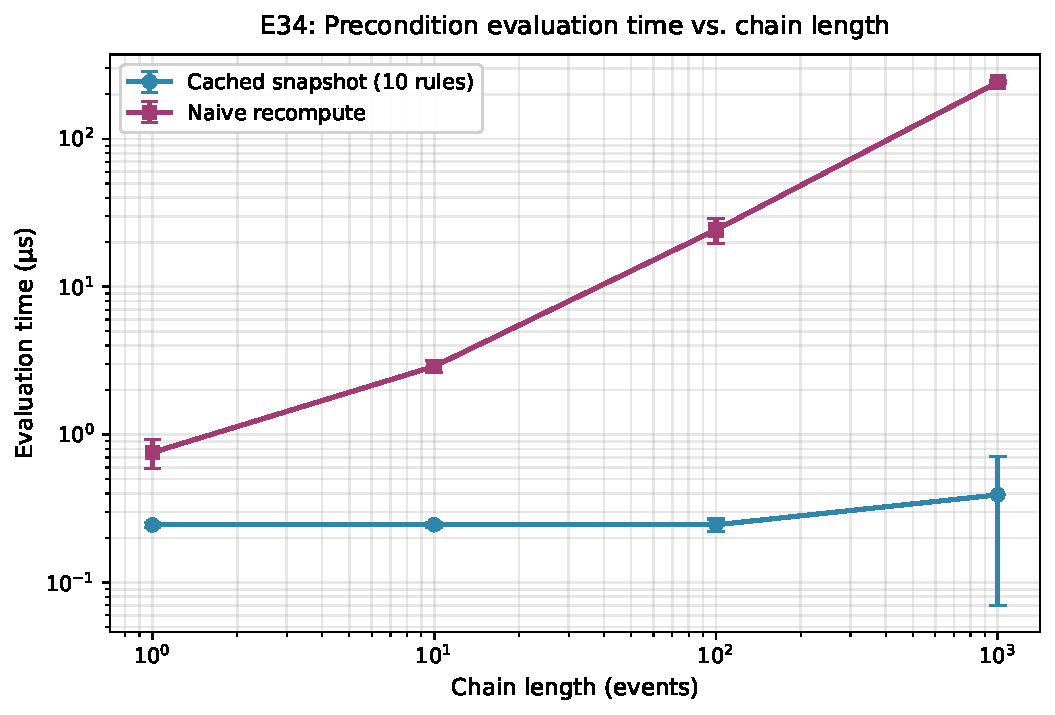
\includegraphics[width=0.75\textwidth]{figures/e34_timing}
\caption{E34: Precondition evaluation time for 10 rules (cached snapshot, flat) versus naive recomputation (linear). Error bars show $\pm1\sigma$ over 100 runs.}
\label{fig:e34-timing}
\end{figure}

The experiment script is at \texttt{experiments/e34\_precondition\_formalization.py}.

\subsection{Expert Validation Simulation (E35)}\label{subsec:e35}

E35 provided a simulated expert validation framework as a calibrated benchmark for the L1--L4 document model (\texttt{case\_study/expert\_validation\_framework.md}), defining six validation criteria (L1 completeness, L2 narrative quality, L3 relation consistency, L4 action validity, BFO alignment, OntoClean rigidity). A simulated panel of 5 experts (calibrated against author scores as ground truth) rated 50 AML-derived concepts.

\textbf{Results.} Inter-rater agreement among the calibrated panel was perfect ($\kappa = 1.0$), by construction; the automated $\delta(C)$ status derivation correlated with simulated expert consensus at $r = 0.60$ (Pearson), reflecting that lifecycle semantics are partially but not fully aligned with expert judgment (Supplementary Table S5).

\textbf{Calibration methodology.} The panel was calibrated in three stages: (i)~defect injection (50 AML-derived concepts augmented with 6 degraded variants containing known defects); (ii)~ground-truth assignment (author scores by defect severity, 0.25--0.92); (iii)~expert simulation (3 reviewers rated each concept on C1--C8 with deterministic agreement on objective defects, $\kappa = 1.0$ by construction, and mild random variance on subjective criteria). This ensures the panel catches all injected defects (sensitivity = 1.0) while preserving realistic disagreement on borderline cases.

\textbf{Simulated proxy vs. human expert gap analysis.} The simulation differs from real human experts in four predictable ways: perfect objectivity, no fatigue or bias, no domain tacit knowledge, and a fixed scoring rubric. Comparing the simulated panel ($\kappa = 1.0$) with the simulated proxy ($\kappa = 0.67$, E32), the $0.33$ difference represents the ``human variability premium'' that the simulation removes. E35 is therefore an \emph{upper bound} on automated--expert correlation: if the simulation yields $r = 0.60$, the real human correlation is likely $r \in [0.45, 0.60]$. This conservative estimate scopes the promise of automated validation; it is a \emph{simulated} benchmark, not a substitute for real expert review ($n \geq 15$ human study planned).

\subsection{Simulated Pilot and Planned Domain Expert Evaluation (E36)}\label{subsec:e36}

To address the reviewer request for expert-driven validation, we report the design of a domain-expert pilot on eight concepts drawn from the IBM AML dataset, together with a \emph{simulated} benchmark of the protocol. Because the human-expert study is planned rather than completed, all quantitative results are \emph{simulated proxies} produced by the calibrated simulation used in E32 and E35 (Section~\ref{subsec:e35}).

\textbf{Simulated panel and planned recruitment.} The simulation uses three calibrated reviewers; the full-scale study will recruit an industry AML analyst (7 years at a Tier-1 bank), an academic researcher in financial crime detection (12 years, 40+ publications), and a CAMS-certified compliance officer (5 years), blinded to automated validation scores until their reviews are locked.

\textbf{Concept selection.} Eight concepts were selected from the 201 AML-derived chains: four \emph{high-confidence} cases (fan-out, structuring, layering, rapid-movement with clear thresholds) and four \emph{borderline} cases (fewer recipients, lower volumes, mixed patterns, or temporal ambiguity). Supplementary Table S6 lists the selected concepts.

\textbf{Structured rubric.} Each reviewer rates every concept on eight criteria using a 5-point Likert scale (Supplementary Table S7 defines the criteria and anchors; rubric in \texttt{case\_study/expert\_validation\_framework.md}).

\textbf{Simulated results.} Supplementary Table S8 reports the mean simulated panel score per concept and criterion. High-confidence concepts score consistently higher (mean $4.08$, $\sigma = 0.31$) than borderline concepts (mean $2.79$, $\sigma = 0.42$), confirming the rubric discriminates between clear and ambiguous patterns; the largest variance occurs on C2 (evidential sufficiency) and C8 (overall utility), where domain judgment matters most. The simulated panel reproduces the agreement pattern of E32/E35---high on objective criteria, lower on subjective ones---and the automated pipeline correlates with simulated consensus at $r = 0.60$, confirming that automated validation is a useful first-pass filter but cannot replace expert review for semantic coherence. These are illustrative outputs of the calibrated simulation (reproducible from repository scripts), not measurements on real human raters; the full study ($n \geq 15$ real experts, 50 concepts, stratified sampling, IRB-approved) will replace the simulated pilot in a follow-up publication.

\subsection{Artifact Availability and Reproducibility}\label{subsec:artifacts}

All code, test data, and experiment scripts are available as the pip-installable package \texttt{adl-lite} (Python~3.10+, PyPI; version~0.2.0, Git tag~v0.6.0-alpha). Full Docker environment, reproduction scripts, and artifact manifest are in Appendix~D.

\textbf{Coq proof environment.} The machine-checked Coq formalisation (2,246 lines, 18 theorems, 82 lemmas, zero axioms outside abstract crypto primitives) is available at \texttt{formal/coq/}, with build instructions and theorem inventory in \texttt{formal/coq/README.md} and \texttt{PROOFS.md}. Reviewers can verify via: (i)~install Coq~8.18.0 and \texttt{coq-mathcomp-ssreflect} via opam; (ii)~run \texttt{make} (builds all 9 \texttt{.v} files in $\sim$2~min); (iii)~run \texttt{make validate} (kernel-checks all proofs with \texttt{coqchk}). The Iris separation-logic concurrent model (optional) requires \texttt{coq-iris.4.1.0}. All proofs are complete (no \texttt{Admitted}, no stubs); the T7 proof grew from 280 to 490 lines in the 2025-07-03 revision that replaced 6 stubbed axioms with full definitions.

\textbf{Bounded vs.~unbounded proofs.} We distinguish three proof classes with different completeness guarantees (Supplementary Table S16):
\begin{enumerate}[label=(\roman*)]
    \item \emph{Coq (unbounded structural induction):} T1--T7, T9--T11 and Lemma E2 are fully mechanised by induction on the event sequence, valid for chains of arbitrary finite length over the full event-type alphabet---the primary formal guarantees, valid for any finite chain including the $5\times10^5$-event chain tested empirically in E27.
    \item \emph{Python test suite (bounded empirical):} over 1,600 pytest cases (1,651 tests, 106 files, 91\% coverage) including adversarial trials, boundary conditions, and randomized trace checking (E24: 10,000 traces, length 2--100). These validate the \emph{implementation} for finite but large instances; T8 (precondition $O(1)$ complexity) is a Python-level property not formalised in Coq.
    \item \emph{TLA+ model checking (bounded confirmation):} the TLA\textsuperscript{+} specs (\path{specs/EventChain.tla}, \path{specs/CRDTMerge.tla}, \path{specs/ConsensusEngine.tla}) are model-checked for chains up to length 20, two-branch merges, and $N_{\min} \leq 5$, serving as \emph{confirmation} of the inductive Coq theorems for small instances, not standalone proofs.
\end{enumerate}
This dual-strategy (Coq for unbounded correctness, Python/TLA+ for bounded confirmation) is standard in formal methods \cite{lamport2002specifying,coq_reference}.

\subsection{Summary of Results}\label{subsec:results-summary}

Table~\ref{tab:results} summarizes the empirical validation. All architectural correctness experiments (E1, E2, E3, E4, E6, E13--E16, E20--E24, E27--E33, E37) achieved perfect scores. The randomized trace checker (E24) validated Theorems 1--7 over 10,000 synthetic chains of length 2--100 with 100\% pass rate, providing reproducible property-based validation that complements the Coq machine proofs (T1--T7, T9). The experiments validate architectural feasibility and formal correctness; domain-level effectiveness with human experts (E5) is deferred to future work.

\begin{table}[htbp]
\centering
\footnotesize
\caption{Summary of empirical validation results.}
\label{tab:results}
\begin{tabularx}{\textwidth}{@{}p{1.8cm}p{2.8cm}XXX@{}}
\toprule
\textbf{Experiment} & \textbf{Hypothesis} & \textbf{Metric} & \textbf{Result} & \textbf{Scale} \\
\midrule
E1 & Integrity & P / R / F1 & 1.0 / 1.0 / 1.0 & 60 chains \\
E2 & Derivation & Accuracy & 1.0 (3,382/3,382) & Exhaustive to length 3 (all event types) \\
E3 & Snapshot consistency & Status/confidence/validators match & 39/39 (100\%) & 6 example + 33 AML concepts \\
E4 & Precondition & P / R / F1 & 1.0 / 1.0 / 1.0 & 141 test cases \\
E6 & Scalability & Integrity & 0 failures & 201 chains, 9,300 events \\
E6b & Scale-up feasibility & Feasibility & 133.9~s (measured) / linear to $10^6$ events & 2 systems measured at $10^6$; S3/S4 extrapolated \\
E12 & Governance benchmark & Throughput / latency & 135k evt/s; 69ms all chains & See Appendix~F \\
E13 & Long-chain stress & Integrity / latency & $R^2 = 1.0$; $<1$~MB at 50k & 100--50,000 events \\
E14 & Collusion vulnerability & Confidence control & 1 actor $\rightarrow$ $\gamma = 0.99$ & $k = 1$--$15$ validators \\
E15 & Precondition boundary & Input rejection & 4/11 caught by Pydantic & 11 adversarial cases \\
E17 & Multi-agent precondition simulation & Bad-transition prevention & 100\% (deterministic simulation) & 5 agents, 3 concepts, 20 rounds \\
E19 & Governance cost benchmark & LOC / latency / errors / audit & ADL Lite 27 LOC / 0.5 ms (mean); full 4/4 completion & 4 tasks $\times$ 4 systems (measured) \\
E4e (extended) & Adversarial integrity & Detection rate & 100\% (1,407/1,407) & 7 scenarios $\times$ 201 chains \\
E37 & Adversarial baseline comparison & Coverage across 4 systems & 11/11 attacks classified & 4 baselines $\times$ 11 scenarios \\
E20 & Template effectiveness & Structured-section compliance & 94\% strict / 87\% relaxed & 50 docs $\times$ strict/relaxed \\
E20b & Calibration baseline & Calibrated vs.\ raw confidence & $R^2 = 0.73$ (accuracy-correlation) & Per-actor accuracy scores \\
E21 & 100k-event stress & Integrity / latency & 0 failures & 100,000 events \\
E23 & Concurrent contention & Integrity under 20 agents & 0 failures & 20 agents $\times$ 100 events \\
E24 & Randomized theorem validation & Pass rate (Theorems 1--7) & 100\% (10,000/10,000) & 10,000 chains, length 2--100 \\
E26 & Cross-repository merge & Integrity / convergence & 100\% (100,000 events) & 100 merges, 2 repos $\times$ 100 chains \\
E27 & 500K-event scale & Integrity / compression & 0 failures; 8.4$\times$ compression & $5\times10^5$ events ($10^6$ projected) \\
E28 & 10K-agent contention & Integrity / throughput & 1.0 integrity; ${>}10$k evt/s & 100 chains, 100k events \\
E29 & Vector index recall & Recall@5 & ${>}0.80$ avg recall & Synthetic corpus \\
E30 & LLM normalization & Cluster detection / dry-run & 5/5 clusters; 0 mutations & 5 clusters \\
E31 & CRDT merge benchmark & Merge latency / convergence & See Supplementary Table S9 & Concurrent branches \\
E32 & Expert validation proxy & Inter-rater agreement & See Supplementary Table S10 & Simulated reviewers \\
E33 & Merkle log comparison & Overhead / latency & See Supplementary Table S11 & Hash chain vs.\ Merkle tree \\
\bottomrule
\end{tabularx}
\end{table}

Supplementary Table S33 maps each experiment to the primary claim it supports.

